% ACS Postdoctoral Fellowship - Fellowship Research Plan (Section 6.1)
% Formatting per ACS General Grant Application Instructions, Sept 2026:
%   - 12pt Times New Roman minimum for text; 10pt for figures, legends, tables
%   - Margins > 0.5 inches
%   - Single or double spaced; if single, blank space between paragraphs
%   - PI name in header on each page; page numbers upper right
%   - 9 pages maximum, excluding references
%
% Compile: pdflatex research-plan.tex  (twice, for the page refs)
%
% ---------------------------------------------------------------------------
% REVISION 23 Nov 2026. Changed passages are wrapped in \chg{...} and print in
% dark blue; \changesfalse below prints them in black.
% STILL OPEN, not applied here:
%   - axis naming drifts: EM axis / EMT axis / epithelial-mesenchymal axis.
%   - Fig 2 panel A axis label renders as "nyori-ness"; regenerate the figure.
%   - no map is stated from model states to the specialties the selection layer
%     filters on; the Fig 1 ordering is asserted rather than derived.
%   - Aim 2's power statement is for a rank correlation; the primary comparison
%     is a difference in explained variance. Not the same test.
% ---------------------------------------------------------------------------

\documentclass[12pt,letterpaper]{article}

% ---------- page geometry: ACS requires > 0.5in margins ----------
\usepackage[letterpaper,margin=0.6in,headheight=15pt,headsep=12pt]{geometry}

% ---------- Times New Roman ----------
% mathptmx = Times for text and math (Nimbus Roman, metrically identical to
% Times New Roman). If you compile locally with XeLaTeX and have the real
% font, swap these two lines for:
%   \usepackage{fontspec}
%   \setmainfont{Times New Roman}
\usepackage{mathptmx}

\usepackage[T1]{fontenc}
\usepackage[utf8]{inputenc}
\usepackage{microtype}

% ---------- header: PI name left, page number upper right ----------
\usepackage{fancyhdr}
\pagestyle{fancy}
\fancyhf{}
\fancyhead[L]{\normalsize Principal Investigator: Hari, Anantha Samrajya Shri Kishore}
\fancyhead[R]{\normalsize\thepage}
\renewcommand{\headrulewidth}{0pt}

% ---------- single spaced with space between paragraphs, per ACS ----------
\usepackage{parskip}
\linespread{0.97}\selectfont
\setlength{\parskip}{4pt plus 2pt minus 1pt}
\setlength{\parindent}{0pt}

% ---------- section headings ----------
\usepackage[explicit]{titlesec}
\titleformat{\section}{\normalsize\bfseries}{}{0pt}{#1}
\titlespacing*{\section}{0pt}{10pt plus 3pt minus 3pt}{3pt}
\titleformat{\subsection}{\normalsize\bfseries\itshape}{}{0pt}{#1}
\titlespacing*{\subsection}{0pt}{8pt plus 2pt minus 2pt}{2pt}

% ---------- float placement: no float-only pages, figures ride at page top ----------
\renewcommand{\topfraction}{0.95}
\renewcommand{\bottomfraction}{0.4}
\renewcommand{\textfraction}{0.06}
\renewcommand{\floatpagefraction}{0.85}
\setlength{\textfloatsep}{10pt plus 2pt minus 2pt}
\setlength{\intextsep}{10pt plus 2pt minus 2pt}

% ---------- tables, figures, links ----------
\usepackage{booktabs}
\usepackage{array}
\usepackage{graphicx}
\usepackage{caption}
\captionsetup{font=footnotesize,labelfont=bf,skip=4pt}   % 10pt for legends
\usepackage{enumitem}
\setlist{nosep,leftmargin=*}
\usepackage[hidelinks]{hyperref}

% ---------- references: numbered, in order of appearance ----------
% ACS wants title, all authors, journal, volume, pages, year.
% unsrtnat numbers in order of first citation and prints full author lists.
\usepackage[numbers,sort&compress]{natbib}
\bibliographystyle{unsrtnat}
\setlength{\bibsep}{4pt plus 1pt}

% ---------- toggle: internal notes, OFF for submission ----------
\newif\ifnotes
\notestrue           % \notesfalse before producing the submission PDF

% ---------- toggle: portal text fields, OFF for submission ----------
\newif\ifstatements
\statementstrue      % \statementsfalse before producing the submission PDF

% ---------- toggle: mark the 23 Nov revisions, OFF for submission ----------
\usepackage{xcolor}
\newif\ifchanges
\changestrue         % \changesfalse prints the revised passages in black
\definecolor{chgcolor}{RGB}{0,70,140}
\ifchanges
  \newcommand{\chg}[1]{\textcolor{chgcolor}{#1}}
\else
  \newcommand{\chg}[1]{#1}
\fi

% ---------- shorthand ----------
\newcommand{\lead}[1]{\textbf{#1}}

\begin{document}

\begin{center}
{\large\bfseries Functional characterization of hybrid E/M plasticity and its link to metastatic potential}
\end{center}

\vspace{2pt}

\section{A. Specific Aims}

\chg{Hybrid epithelial/mesenchymal phenotypes have been associated with tumor-initiating and metastatic behavior in several carcinoma models \cite{jolly2019,pastushenko2018}. Cells in these hybrid states co-express epithelial and mesenchymal markers. That combination is thought to allow collective migration, as small clusters of circulating tumor cells.

Work over the past decade has added plasticity to this picture: the ability to change phenotype reversibly under environmental perturbation. Plasticity is held to raise metastatic potential by increasing population heterogeneity. It is usually measured on one axis, repopulation efficiency, meaning how much heterogeneity a sorted population recovers in vitro or in vivo \cite{gupta2011,pastushenko2018,ruscetti2016,brown2022}. High plasticity of hybrid states has therefore been read as low stability to perturbation.

Three observations resist that reading. First, transcriptomic measurements of hybrid states consistently return heterogeneous populations. Earlier work attributed this to metastability. More recent work has established stable hybrid lines \cite{kroger2019} and has shown that hybrid-state heterogeneity predicts worse outcome \cite{brown2022}. Second, hybrid phenotypes carry pro-metastatic features, among them stemness, drug resistance and immune evasion \cite{mani2008,sahoo2021}. Under the classic account a perturbed hybrid cell loses its identity, and those features go with it: driving hybrid cells to a fully mesenchymal state removes their tumor-initiating capacity \cite{kroger2019}. Third, no clean molecular signature of the hybrid phenotype exists, unlike the signatures for E and M. That has kept these associations from translating, and it leaves an open question: is there a limited set of hybrid phenotypes, or a continuum?

Holding the three together calls for a characterization that low-dimensional measures cannot supply. EMT scores and heterogeneity indices compress high-dimensional transcriptomic data to one number \cite{tan2014,george2017,mroz2013}. Static measurements such as transcriptomics also cannot faithfully capture dynamical properties such as plasticity.

We propose two quantities, computed on Gene Regulatory Network (GRN) models. Each is defined against a stated perturbation, a starting state, a boundary for the hybrid phenotype, and an observation window. Retention is the share of the window a trajectory spends inside the hybrid phenotype. Reach is the number of distinct hybrid states it visits, as a fraction of those available at matched state-space size. The hybrid phenotype is bounded by the EMT score together with the constraint that the marker combination permitting collective migration is held; Aim 1 states the definition and the conditions under which it would be revised.

Together the two span a plane, and its corners name three regimes. Low retention is metastable: a hybrid cell leaves readily and settles at one extreme. High retention with low reach is stable: a cell holds one hybrid state. High retention with high reach is a cloud: a cell moves among hybrid states while the phenotype persists. Networks are placed in the plane and intermediate cases are reported. Which regimes a network can access is a property of the network. Noise decides which one is expressed, so Aim 1 records the set rather than the behavior at one noise level. Networks are general and are not fitted to individual lines, so the match to a cell line is qualitative. Stabilized hybrid lines instantiate the stable regime. Lines that resolve to pure E or pure M instantiate the metastable one. Lines in the cloud regime are what this project predicts and sets out to identify.}

The regimes should not be equally metastatic. Metastasis makes conflicting demands in turn, requiring shear resistance and immune evasion in transit and re-epithelialization at colonization \cite{jolly2019}, and clusters of circulating tumor cells seed far more efficiently than single cells \cite{aceto2014}. \chg{Each demand removes the cells not equipped for it, so for a population of cells with fixed specialties the demands compound, and survival is the share of cells that happen to carry every specialty the sequence calls for. A population whose cells move among hybrid states re-equips between demands, so the survivors of one are available to the next and the sequence does not compound in the same way. This requires no coordination between cells, only movement on a timescale comparable to the interval between demands.} Figure~\ref{fig:regimes} sets out the predicted orderings. The two are indistinguishable in a snapshot on any number of axes, which is what makes a dynamical measurement necessary.

\lead{Central hypothesis.} Epithelial-mesenchymal plasticity comprises distinguishable dynamical regimes that differ in reach and retention, and the regimes a cell can access predict its metastatic competence better than its position on the epithelial-mesenchymal axis alone.

\lead{Aim 1. Fix the regimes, their signatures, and what they imply for survival.} Reach and retention are computed on the state-transition graphs of multilevel EMT networks, across a noise sweep and at matched state-space size. The same computation fixes what Aim 2 depends on: the observation window each assignment requires, and the projection of model states onto a marker panel. A selection layer then applies the stresses of transit and colonization to simulated trajectories in small groups. The layer can show that the phenotypic framework does not produce survival under plausible filters, or that it does not separate the regimes. Either outcome identifies what the model is missing.

\lead{Aim 2. Test the regimes in cells and against metastatic outcome.} Existing single-cell data and functional assays establish whether hybrid cells carry distinct specializations. Across roughly 30 mouse and human lines, cells are then sorted on one property and re-assayed on another over time, which separates a mixture of committed cells from a population that converts between states, and a TGF-$\beta$ dose series measures response steepness per line. Fourteen of these lines have been through orthotopic and tail vein metastasis experiments, so regime assignment is tested against those outcomes with baseline hybrid fraction as the competing predictor. Live imaging then measures transitions in single cells over the window Aim 1 specifies.

\lead{Aim 3. Genetic and epigenetic mechanisms of the heterogeneity in plasticity.} \chg{Two} candidate mechanisms for what makes regulation graded are tested against regime assignment: intermediate DNA methylation at EMT regulatory elements\chg{,} and microRNA-mediated buffering. Each predicts a different pattern of gradedness across the circuit, which is what makes them separable.

Aims 1 and 2 together test the central hypothesis, and Aim 3 builds on them.

\section{B. Background and Significance}

The axes are not independent, which is what makes a one-dimensional score lossy. EMT generates cells with the properties of stem cells \cite{mani2008}, and a model in which EMT and drug resistance are coupled predicts hybrid cells that are drug-sensitive and hybrid cells that are drug-resistant, switching stochastically between them \cite{sahoo2021}. The same trade-off appears outside EMT, where HMGB2 sets the balance between proliferative and invasive melanoma states and cells pushed toward the invasive state divide less and tolerate drug better \cite{hunter2025}. Two cells at the same position on the EMT axis can therefore differ in what they are equipped to survive. The claim this project makes is narrow. A transcriptomic metric can already separate genuine hybrid cells from a mixture of epithelial and mesenchymal cells \cite{chakraborty2020}, a comparison resolved along the EMT axis and not within one position on it. What has not been tested is whether a single population moves among hybrid states, or whether that movement, as distinct from composition, predicts outcome. \chg{The regime signatures, the observation window and the marker panel are all fixed by the model before the cells are sorted.}

\lead{Relevance to cancer.} The hybrid E/M state is strongly associated with metastatic competence and therapy resistance across carcinomas \cite{jolly2019}. Successful completion of this work would establish whether the clinically relevant property of that state is compositional, as currently measured, or dynamical. This project does not deliver an assay for patient tissue. It establishes whether the quantity is worth measuring, and identifies which molecular features track the regime, which is what any attempt to move a tumor from one regime to another would have to target.

% ---------------------------------------------------------------
% ---------------------------------------------------------------
\begin{figure}[!t]
\centering
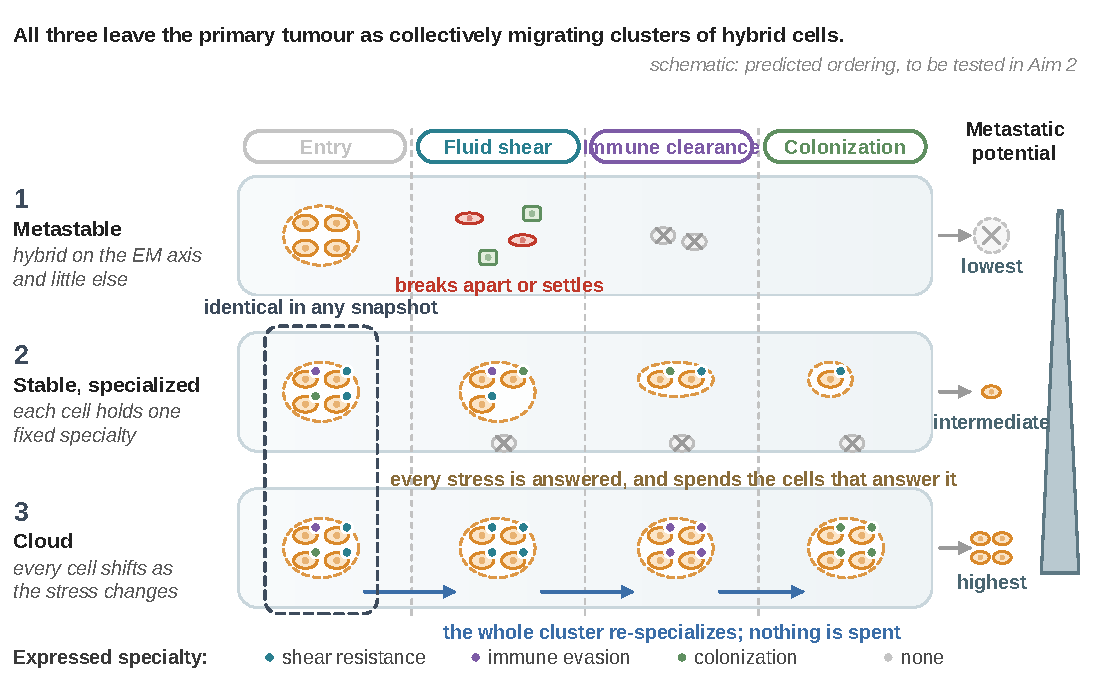
\includegraphics[width=0.96\textwidth]{Fig1.pdf}
\caption{\textbf{What separates the regimes is what a cluster can do when the \chg{demands change}.} All three leave the primary tumor as collectively migrating clusters, so cohesion at the outset does not distinguish them. A metastable cluster is hybrid on the EM axis and little else, and breaks apart at the first \chg{demand}. \chg{In a cluster of cells holding fixed specialties, each demand removes those not equipped for it, so the demands compound and the cells that remain are rarely the ones the next demand calls for. A cluster whose cells move among hybrid states re-equips between demands, which requires no coordination between cells, only movement on a timescale comparable to the interval between them.} Rows 2 and 3 carry the same composition on any measured axis, so any index computed from one timepoint returns the same value for both. The potential column is an ordering and not a magnitude: it is what the selection layer in Aim 1 predicts, to be tested against the metastasis data in Aim 2, and higher metastatic potential is the direction that would correspond to worse patient prognosis.}
\label{fig:regimes}
\end{figure}

\section{C. Preliminary Studies}

\lead{Attribution.} The simulation results below were generated by the applicant. The flow cytometry panels, the orthotopic metastasis screen, the inducible constructs and the single-cell sequencing referred to throughout were generated by the Mani laboratory (Brown University) and are used here with permission; no part of that work is claimed as the applicant's own.

\chg{Hybrid states are the ones a network holds least firmly. Across 13 EMT and EMP networks under single-edge perturbation, hybridness and multistability trade off, and the correlation is negative in 12 of them (Fig.~\ref{fig:prelim}A) \cite{rashid2022}.

Gene regulation is usually modeled as binary, in Boolean models or in sigmoidal ODEs. Under binary regulation a hybrid state requires opposing regulators to be simultaneously satisfied, which they cannot be, and the state inherits that conflict as instability. Allowing a gene to take intermediate levels relieves it. We find that the same 23-gene EMT network, given identical starting states and identical noise, behaves in two ways depending only on how many levels each node takes (Fig.~\ref{fig:prelim}B). Under binary regulation cells leave the hybrid band. Under graded regulation they move within it and the population stays hybrid. The in-band fractions, 15 against 52 percent at low noise and 67 against 98 at high noise, are retention as defined above, measured on these runs.

Individual hybrid states remain sensitive to perturbation in both implementations. What differs is where a perturbed cell goes. Under graded regulation it moves to a neighboring hybrid configuration, so the phenotype persists while the states turn over. That is the cloud regime. Graded regulation also produces fixed points absent from the binary model, with roughly half of settled cells landing on states the binary catalog does not contain, and the two implementations separate several-fold only when perturbations preserve their magnitude and the network is left to relax between them. These runs apply a fixed intermediate level uniformly to the graded nodes, so they establish that the cloud regime can arise from gradedness in this network under a stated perturbation regime. How much gradedness is needed, and where it has to sit, is what Aim 1 takes up.}

\begin{figure}[!t]
\centering
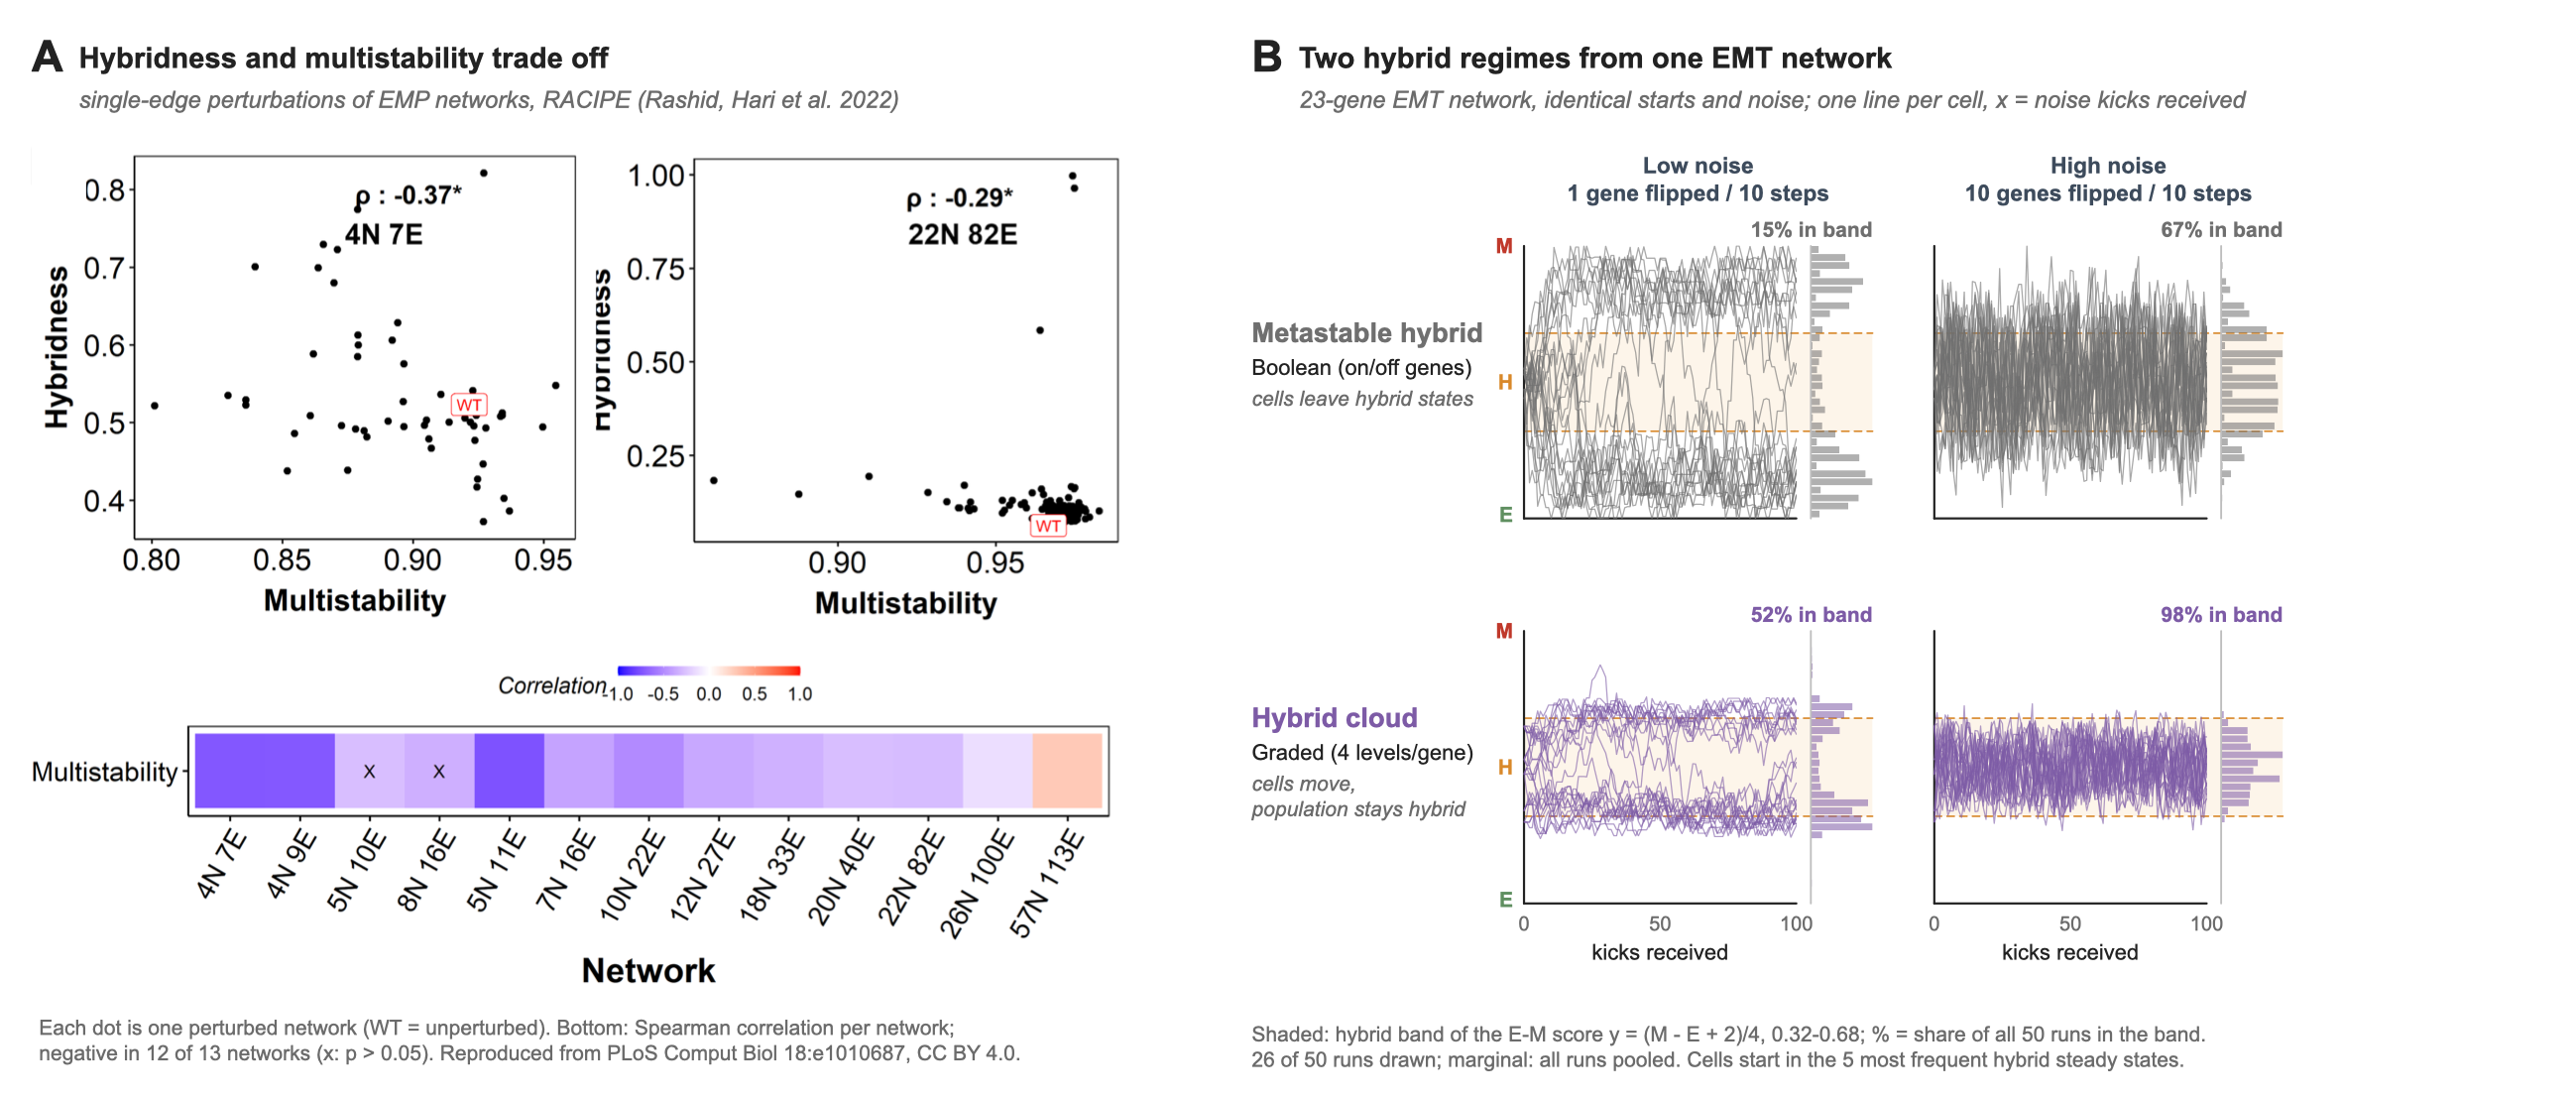
\includegraphics[width=0.97\textwidth]{Fig2.png}
\caption{\textbf{Preliminary results.} (A) Across 13 EMT and EMP networks under single-edge perturbation, hybridness and multistability are negatively correlated, significantly so in 12 of the 13; two example networks are shown with the unperturbed network marked. Reproduced from our published analysis \cite{rashid2022} under CC BY 4.0. Hybrid states are therefore the ones a network holds least firmly, which is what makes their dynamics worth separating. (B) The same 23-gene EMT network under two-state and graded regulation, started from identical states and given identical noise, with one line per cell and the pooled distribution against the right edge of each panel. Under two-state regulation cells leave the hybrid band; under graded regulation they move within it and the population stays hybrid, at both noise levels tested. The in-band fractions quantify this. \chg{The in-band fractions are retention measured on these runs. Both regimes arise from one network, which is what the classification in Aim 1 formalizes.}}
\label{fig:prelim}
\end{figure}

\section{D. Research Design and Methods}

\subsection{Aim 1. Fix the regimes, their signatures, and what they imply for survival}

\lead{Rationale.} Regimes remain a model construct until each predicts something a cell can be observed doing, and those predictions must be fixed before any cell is sorted or Aim 2 becomes an exercise in fitting. Three quantities are fixed here: the regimes each network can access, the observation window an assignment requires, and the markers it is read on.

\chg{\lead{What counts as the hybrid phenotype.} Reach and retention are both defined against a set of hybrid states, so that set is fixed before either is computed. It starts from the EMT score, as the band between the epithelial and mesenchymal extremes, with one constraint added: the marker combination that permits collective migration must be held. A state inside the score band that has lost that combination is outside the phenotype. Collective migration is read indirectly in the panel in hand, from cluster counts and the wound healing assays; the migration assay requested below would measure it directly. The definition is provisional. If the mass cytometry data show that other functional properties travel with the hybrid state, the constraint set can be widened to include them and both quantities recomputed. Revising the boundary is not an aim of this project, and every result reports the definition it was computed under.}

\lead{Regimes as capacities of a network.} Reach and retention are computed on the state-transition graph of a multilevel EMT network, which lists the states a cell can occupy and the moves available from each. \chg{Retention is the share of the observation window a trajectory spends inside the hybrid phenotype, averaged over trajectories started from hybrid states. Reach is the number of distinct hybrid states it visits, as a fraction of those available at matched state-space size. Both are fractions, so they can be compared against measured trajectories without mapping a model step to an interval of real time. Low retention is the metastable regime, high retention with low reach the stable regime, and high retention with high reach the cloud regime. A trajectory can hold high residence across two states or across forty, so neither quantity determines the other; whether they come apart across the ensemble is what the dissociation test asks.} Retention is a model quantity, and it predicts that the functions the hybrid phenotype supplies are preserved while a cell moves within it. Collective migration is the clearest of those, since it requires neighboring cells to hold compatible adhesion states, and the mass cytometry panel supplies others measured in the same cell, including stemness, apoptotic state and hypoxia response. High retention therefore predicts a set of preserved functions, so a single disagreeing assay does not settle the question. Noise moves a network between regimes, since a cloud population at low enough noise settles and resembles a mixture of stable cells, so noise is swept across its range and the regimes that appear are recorded. Comparisons are made at matched state-space size, since a four-level network has more states than a two-level one for arithmetic reasons alone. An ensemble of EMT topologies is run this way, each in graded and two-state form, so gradedness is the only property varying within a pair.

\lead{The observation window.} A metastable trajectory also moves among hybrid states before it exits, so too short a window makes it resemble a cloud trajectory. The distribution of transitions before exit sets a minimum window, and Aim 2 anchors that window in hours using the reference lines described there.

\lead{Projection onto a measurable panel.} Model states live in gene space and flow cytometry reads markers, so reach and retention are computed in the projection onto a candidate marker set. Running several networks covering different pathological contexts yields a marker set that keeps the regimes separable, and the smallest number of channels that does so. That set is checked against the mass cytometry data already in hand, in which functional markers and EMT markers are measured in the same cell. Agreement supports the projection; disagreement indicates regulation the data resolve and the networks omit, and identifies which networks to revise.

\lead{A selection layer that tests the framework.} Reach and retention say nothing about whether a cell survives getting anywhere, and the stages between primary tumor and metastatic site kill most cells that attempt them. A selection layer is therefore applied to trajectories in small groups, with the network and regime definitions held fixed. Most suspended breast tumor cells are killed by fluid shear, and survivors are enriched for mesenchymal and hybrid phenotypes, with shear inducing EMT through JNK signaling \cite{xin2020}; survivors are also softer \cite{xin2019}, and epithelial-like and mesenchymal-like lines differ under the shear and constriction of the microcirculation \cite{cognart2020}. Confinement is not only a filter but a cue that switches state through chromatin \chg{remodeling} \cite{hunter2025}, which is why the layer acts on trajectories that can still move. A Boolean model integrating hypoxia, mechanosensing and TGF-$\beta$ signaling reproduces state changes across the metastatic cascade \cite{greene2025} and supplies the signaling scaffolding, representing neither immune clearance nor survival at the level of a group.

\chg{Filters are probabilistic rather than absolute, and each represented state answers its own demand and, to a degree that is varied, demands adjacent to it. That breadth decides how steeply the regimes separate: with narrow states the demands compound and a population of fixed specialties is depleted quickly, while with broad states such a population can meet the whole sequence and the predicted ordering flattens. Breadth is therefore swept alongside filter strength, and the range over which the ordering holds is reported rather than a single value.} Each regime yields a fraction of groups surviving transit and then meeting the re-epithelialization demand, and the predicted ordering is what Figure~\ref{fig:regimes} sets out. Three outcomes are possible. The ordering holds, which derives the schematic from the model. The regimes do not separate under the filters, which means the framework does not carry the survival claim. Or no regime survives at plausible filter strengths, which would mean the represented phenotypes are insufficient and would identify the missing axis. Filter strength is swept across its plausible range, since kill rates are not well constrained.

\lead{What the perturbation has to be.} Separation depends on how far a perturbation moves a node and on how much time passes between perturbations. Perturbations too small leave graded and binary networks alike, and perturbations faster than the network settles leave every implementation looking hybrid on a team-averaged coordinate, which is a property of the average and not of the state. Retention is therefore scored on the condition that node levels persist between perturbations. Reversing the sign of a node's level is directional by construction, so the sweep is repeated with random-sign perturbations of matched magnitude.

\lead{Statistical analysis.} The unit is a network, since the model carries no kinetic parameters and what varies between lines is which links are graded. Networks are compared by the set of regimes the noise sweep returns, not by a value at one noise level. Separability is the proportion of networks whose reach and retention place them in one regime with no overlap against the adjacent range, with bootstrap intervals over the ensemble. Effect sizes replace significance tests, since ensemble size is set by computation. The dissociation test asks whether reach and retention are correlated across the ensemble; a rank correlation near unity would indicate a single underlying axis. \chg{Retention is reported against an entropy-matched null, the same phenotype boundary and state-space size under regulation-free dynamics, since more configurations map to intermediate EMT scores than to the extremes and residence would be high there on combinatorics alone.}

\lead{Expected outcomes and benchmarks.} There is no precedent for setting a separability threshold in advance, so it will be fixed from the first ensemble and reported before any regime is assigned in cells. Networks falling between regimes are reported, not discarded, since intermediate cases are what continuous gradedness would produce. The second benchmark comes from runs already performed: graded networks should hold the hybrid phenotype several times more often than binary networks of the same topology under perturbations allowing relaxation, and that gap should close when perturbations are too small or too rapid. For the selection layer the benchmark is robustness, that the predicted ordering holds across the filter sweep\chg{ and over a stated range of state breadth}.

\lead{Potential problems and alternatives.} The classification fails if the regimes collapse onto a single axis once state-space size is matched, and that outcome is reported. The dissociation between reach and retention is unconfirmed and central to the cloud regime, so testing it is the first task. If the two cannot come apart, the project reverts to a graded against switch-like comparison, which the dose series still tests.

\subsection{Aim 2. Test the regimes in cells and against metastatic outcome}

\lead{Rationale.} A population measured once cannot distinguish a mixture of committed cells from a population that converts between states. Sorting a subpopulation and watching it re-equilibrate separates the two, and this design established stochastic state transitions in breast cancer lines \cite{gupta2011}. \chg{What the existing measurements lack is not markers but a time axis: the flow panels and the mass cytometry measure many properties in single cells at one moment, and the one assay that does follow a population over time reads it on a single epithelial-to-mesenchymal coordinate. Retention predicts that a set of functions is held together while a cell moves within the hybrid band, which a one-dimensional readout cannot address and a snapshot of many markers cannot either.}

\lead{What runs before the sorting work.} Mass cytometry already run on these models measures functional properties in the same cell as the epithelial and mesenchymal markers, covering stemness, apoptotic state, hypoxia, cell cycle and signaling, and establishes whether hybrid cells carry distinct specializations, which the mixture condition requires. Existing single-cell transcriptomics covers two models at one timepoint and checks marker behavior there. Either answer is informative: discrete specializations give a mixture to contrast the cloud regime against, continuous ones supply the variable for ranking lines. Public resources such as CCLE carry regime assignment beyond the panel in hand.

\lead{Reference lines with known behavior.} Lines that do not hold a hybrid state after induction supply a metastable reference, and established stable hybrid lines supply a stable one. Hybrid cells isolated from each are followed until they re-equilibrate, which validates the assay on the existing low-dimensional panels, anchors the observation window from Aim 1 in hours, and brackets the retention axis from both ends, so the cloud regime is identified by exceeding both references in reach while matching the stable reference in retention.

\lead{Approach.} Paired flow panels across roughly 30 mouse and human lines score cells as epithelial, hybrid or mesenchymal at baseline, after TGF-$\beta$, and after receptor inhibition. Cells are sorted on one property and re-assayed on the other, then re-assayed on the first over time. The regimes predict different outcomes, as Figure~\ref{fig:regimes} sets out: a stable hybrid population stays sorted, a metastable one re-equilibrates across the full range, a cloud population re-equilibrates within the hybrid range alone. TGF-$\beta$ is also titrated across a dose series, with response steepness measured per line, since transition rates depend on the dose and duration of EMT-inducing signals \cite{subhadarshini2023}. A dose series is a sustained directional input, corresponding in the model to perturbations slow enough for the network to settle, so its range must span magnitudes large enough to move a node. \chg{Per-cell time and many markers do not come together in one assay, so each level answers a different part of the prediction. Population re-equilibration after sorting separates a converting population from a committed one. The multi-marker panel read at intervals across that re-equilibration tests whether the set of functions retention predicts is preserved while cells move. Reporter imaging supplies per-cell rates in the lines where reporters exist. The aim reports which level each conclusion rests on.} Sorting hybrid populations and following how the ratios regenerate is already under way in the collaborating lab. This aim adds the prior classification: \chg{the signature each regime predicts, the window it is read over and the markers it is read on are fixed in Aim 1 and registered before any re-equilibration or dose-response result is examined.} A sorting experiment on its own measures how fast ratios return. With \chg{that mapping} registered in advance it tests whether the regimes are real.

\lead{Metastatic outcome, against hybrid fraction.} The classification is useful only if it predicts an outcome that position on the EMT axis does not. Fourteen mouse lines have been through an orthotopic screen with circulating tumor cell colony counts. Regime assignment is tested against these outcomes with baseline hybrid fraction entered as the competing predictor, not as a covariate. The same lines have been through tail vein injection, which bypasses the primary tumor, so comparing the two entry points discriminates where regime acts: stronger prediction of the tail vein outcome places the effect in transit and seeding, where the selection layer puts it, and stronger prediction of the orthotopic outcome places it at escape. Clustered circulating tumor cells are disproportionately efficient seeds \cite{aceto2014}, and cluster counts are the closest available readout of the collective migration that high retention predicts, so they are designated in advance as the primary test, with total burden secondary and the existing wound healing assays as the in vitro correlate, and the selection layer's predicted ranking of regimes by surviving fraction is fixed before the screen data are examined. \chg{The immune compartment of these tumors differs by EMT class, so this comparison speaks to which lines seed and not to whether the difference is cell-intrinsic.}

\lead{Imaging, where rates are measured directly.} Population distributions before and after a perturbation are not switching rates. Live imaging of reporter lines tracks cells individually through state changes in a subset spanning the assignments, over the window Aim 1 specifies. It is placed last because it is worth doing only in lines whose assignment is settled. The collaborating lab has built ESRP1 and Vimentin reporters in human lines, so this arm runs on the human panel, with regime assignment from the same flow and dose assays as the mouse panel. Where reporters are unavailable the aim reports re-equilibration kinetics, and per-cell rates go unmeasured.

\chg{\lead{Measurements requested of the collaborating laboratory.} Three further measurements would test predictions the panel in hand cannot reach: migration capacity under defined geometry, for which cluster counts are an indirect readout; stress induction other than TGF-$\beta$, which tests whether reach measured under one input predicts the response to another; and co-culture with immune effectors, the demand the selection layer represents least well. Migration, invasion and immune-remodeling assays are established in the collaborating laboratory and were applied to these hybrid models recently \cite{visal2025}, so what is new is the design and not the capability. None is part of the laboratory's current program, and no experiment is charged to this award, which carries no research budget. Each would be requested on the scientific case for it, and making that case is part of the training this fellowship provides. The aims above return a result without them.}

\lead{Statistical analysis and power.} Regime assignment is tested against cluster counts by rank correlation across the fourteen lines, with hybrid fraction in the same model and the two compared by difference in explained variance with bootstrap intervals. Dose-response steepness is estimated per line by fitting a Hill function to the fraction past the hybrid gate, with the Hill coefficient as the statistic. Fourteen lines support detection of a strong rank correlation ($\rho \approx 0.7$\chg{, two-sided, 80\% power, $\alpha=0.05$}) and no more, so this arm is powered and reported as a screen. Lines are the unit for the metastasis comparison, replicate wells for the dose series.

\lead{Expected outcomes and benchmarks.} The benchmarks divide by what each assay resolves. On existing panels, success is the reference lines behaving as predicted, which needs no new data. On a higher-dimensional panel, success is resolving structure inside the hybrid gate, which three bins cannot show. For the comparison against hybrid fraction, success is regime explaining substantially more variance in cluster counts, reported as a difference with its interval; with fourteen lines a small difference supports no claim either way, so the benchmark is a substantial difference or none.

\lead{Potential problems and alternatives.} The three-color panels score one axis, so telling a cluster of specialists from a cloud needs several specialization markers on the same cell. Raw intensities are retained as a matter of course and give resolution within each channel but not extra channels, so the first check is whether the mass cytometry panels already run on these models carry the markers the Aim 1 projection calls for; where they do not, a panel is designed from that projection and the dose series carries the aim meanwhile. Cell-to-cell variation in receptor level can also flatten a dose response, and that alternative is tested by measuring steepness in single cells, not population means. \chg{Perturbations achievable in culture may also be too small to reveal the reach a cell has in vivo, so the dose range is reported against the magnitude the model requires, and a null result is read as insufficient perturbation rather than absent reach.} The hypothesis fails if sorted hybrid populations in cloud-assigned lines re-equilibrate across the full range, if steepness is unrelated to assignment, or if hybrid fraction predicts cluster counts at least as well. Fourteen lines cannot establish that regime is uninformative, so a null is reported as the limit of the panel's power.

\subsection{Aim 3. Genetic and epigenetic mechanisms of heterogeneity in plasticity}

\lead{Rationale.} Aims 1 and 2 establish that regimes exist and track outcome. Neither says what makes one cell's regulation graded and another's switch-like. Without that, regime is a label a cell is assigned, and not a property that can be moved. What produces an adaptive cell state remains an open question, with recent proposals placing it in stress-responsive machinery carrying regulatory combinatorics and cellular memory \cite{franca2026}.

\lead{From a mechanism to a network property.} A mechanism that correlates with a regime label explains nothing on its own. The model needs a mapping from mechanism to the property that sets the regime, which here is which links are graded. Epigenetic regulators compete globally for targets, so a change in one redistributes marks and alters the EMT landscape in ways local models do not capture \cite{alradhawi2022}. That supplies the route from a methylation change to a change in how graded a link is. Two mechanisms are tested, and they predict different patterns of gradedness, which makes them separable. Intermediate DNA methylation can act globally or at particular elements, and which applies is testable; locally disordered methylation dominates intratumor methylome variation, accompanies low-level expression and tracks worse outcome \cite{landau2014}. MicroRNA-mediated buffering acts on miR-200 family targets, so the gradedness it produces is concentrated on the mesenchymal side of the circuit; the miR-200/ZEB circuit behaves as a ternary switch driven by miR-34/SNAIL, which acts as a noise-buffering integrator \cite{lu2013}. Asking which patterns reach the cloud regime at all is a model question Aim 1 can answer, and it turns how much gradation is needed into how much and where.

\lead{Approach.} Read-level methylation disorder at EMT regulatory elements is scored against regime assignment across lines, on public cell-line resources for the human panel where such data exist. Equivalent data for the mouse syngeneic lines is not assumed: whether it exists is checked in the first months, and if not the analysis runs on human lines alone. For the microRNA arm, inducible miR-200 and ZEB1 lines exist in D2A1 and EMT6 and have been through metastasis experiments in the collaborating lab, \chg{where inducing either reduces lung metastasis}. No new perturbation is proposed\chg{ by this award}. \chg{Following the multistate treatment of microRNA regulation in \cite{lu2013}, miR-200 dosage is varied in the model, which predicts where in the dosage range gradedness peaks and therefore which dosage should maximize retention within the hybrid band. That is a location and a shape a composition account does not fix, and it is what a titration in the inducible lines would test; such a titration is a request to the collaborating laboratory rather than something this award funds.} This analysis forms part of a collaborative manuscript in preparation with that laboratory, and the fellowship would fund the modeling and the analysis, not the experiments.

\lead{Statistical analysis, power and benchmarks.} Each mechanism is entered as a predictor of regime assignment across lines, with both in one model so shared variance is visible. This is a correlational screen across roughly 30 lines, so no power calculation on a treatment effect applies, and it is reported with effect sizes and intervals. Success is at least one mechanism tracking regime assignment, a gradedness pattern matching the one it predicts, and, for the microRNA arm, \chg{the model predicting the dosage at which retention within the hybrid band is highest. The existing result that induction in either direction reduces metastasis serves as a consistency check and not as the test, since a composition account predicts it equally well.}

\lead{Potential problems and alternatives.} Correlation between a mechanism and a regime does not establish that the mechanism produces it, and the microRNA arm tests a prediction against a completed perturbation. \chg{ZEB1 induction also induces dormancy in these lines in vitro, so reduced metastasis after induction carries a proliferation explanation alongside the plasticity one, and the predictions this arm makes are chosen to be ones dormancy does not also produce.} The aim fails if neither mechanism tracks regime assignment, which would place gradedness outside this list, most likely in chromatin accessibility. That outcome is reportable and narrows the field.

\lead{Relation to other funded work.} The modeling framework above arose from work supported by an active award on EMT and stemness held jointly by the mentor and the collaborating laboratory. That award asks how epigenetic control shapes the stemness axis. This aim asks what sets gradedness in the EMT circuit and whether it determines plasticity regime, a different question on a different axis, and no specific aim is shared.

\subsection{Feasibility, timeline and risks}

The first two years run on existing material and the third buys the measurement the first two cannot make. The modeling code exists and has produced the preliminary results, the flow panels and the metastasis experiments have been run, and no aim requires a new animal cohort. Aim 1 occupies the first six months, beginning with the reach-and-retention dissociation that the rest depends on, and delivers the fixed signatures before any cell is sorted. Aim 2 runs from month four to month \chg{twenty-two}: the check on existing panel coverage in month four, the dose series as soon as it returns, and the metastasis analysis from month eighteen once assignments exist. Aim 3 \chg{opens at month twenty, in the last stage of year two, with the mentor overseeing how the mechanism work is planned}. Nothing is blocked: the dose series does not wait on the sorting experiments, and the methylation analysis does not wait on either. \chg{Year three is led by the applicant: building the mechanism model, running the analysis, and requisitioning the experiments the model calls for, with any request to the collaborating laboratory placed during year two so that its lead time does not consume the final year. The imaging arm runs here, in the lines whose assignment is settled, and the dose-response, metastasis and mechanism comparisons are completed and reported by month thirty-six.}

\begin{table}[htbp]
\centering
\footnotesize
\begin{tabular}{@{}p{0.26\textwidth}p{0.26\textwidth}p{0.42\textwidth}@{}}
\toprule
\textbf{Risk} & \textbf{What it costs} & \textbf{Response} \\
\midrule
Reach and retention do not dissociate in simulation & The three-regime scheme reduces to two & Tested first, in month one; the project reverts to a graded against switch-like comparison, which the dose series still tests \\
\addlinespace
Existing panels measure too few markers at once & A cluster of specialists cannot be told from a cloud & Mass cytometry panels already run on these models are checked first; where they fall short, a panel is designed from the model's projection \\
\addlinespace
TGF-$\beta$ was applied at a single dose rather than titrated & No existing data speak to steepness & A new dose series is the default plan, and is a request to the collaborating lab, not something this award funds \\
\addlinespace
Reporters exist only in human lines & Per-cell rates cannot be measured in the mouse panel & The imaging arm runs on the human lines, with regime assignment from the same assays; elsewhere the aim reports re-equilibration kinetics and says rates were inferred \\
\addlinespace
Fourteen lines detect only a strong effect & The metastasis arm cannot rule regime out & Powered and reported as a screen; the model and cell arms stand independently \\
\addlinespace
Analyses of the collaborating lab's data may already be committed & Duplicated or contested work & Resolved before submission by asking which analyses are unclaimed \\
\bottomrule
\end{tabular}
\end{table}

\section{E. Impact}

A single number collapses two questions into one: what produces heterogeneity in a tumor, and what it does once present. Treating plasticity as multidimensional separates them. The regimes proposed here differ in mechanism, in what they predict under successive demands, and in metastatic competence, while returning the same value to any index computed at one timepoint. If they can be told apart in cells, the field gains a description of a tumor cell population that composition cannot supply.

The methodological contribution is a pair of quantities computed on a network and read on a marker panel the same model specifies, which gives the modeling literature on EMT predictions that a flow cytometer can refute. The project also leaves behind a model in which the survival of a group of cells depends on the plasticity regime of its members, which existing models of the cascade do not represent. The clinical route runs through Aim 3, not Aim 2. A perturbation assay is within reach for patient-derived lines \cite{brown2022}, but a biopsy is a single timepoint, so an assay that scales to routine samples has to be static. \chg{What tracks} gradedness, which Aim 3 asks, would supply a static signature for a dynamic property.

\clearpage
\small
\bibliography{references}

\ifnotes
\clearpage
\section*{Appendix: ACS requirements for this document}
\addcontentsline{toc}{section}{Appendix}
\small

Internal checklist, compiled from the ACS General Grant Policies and the General
Grant Application Instructions, both effective September 2026. Not part of the
submitted proposal: set \texttt{\textbackslash notesfalse} in the preamble to
drop this appendix before export. Page numbering restarts nowhere, so removing
it leaves the body pagination unchanged.

\subsection*{A. The research plan itself (Section 6.1)}

Nine pages maximum, excluding references. The plan must be realistic for the
period of support requested, and a timeline is encouraged. Six required
elements, in this order:

\begin{enumerate}
\item \textbf{Specific Aims.} List the objectives and goal of the research
  proposed, and describe the specific aims briefly, in order of priority.
\item \textbf{Background and Significance.} Concisely summarize and critically
  evaluate relevant work done by others that provides a rationale or
  justification for the project. State specifically how successful completion
  of the work will advance scientific knowledge relevant to cancer initiation,
  prevention, detection, treatment or survivorship.
\item \textbf{Preliminary Studies.} Optional. If included, give results of
  research accomplished by the applicant or others that is relevant to the
  proposal, explain its significance to the scientific rationale, and
  \emph{carefully attribute the source of any preliminary data}.
\item \textbf{Research Design and Methods.} Methods and procedures in
  sufficient detail to permit evaluation by other scientists. Must include: a
  statistical analysis plan; a power analysis to support design and sample size
  where applicable; expected outcomes and anticipated benchmarks for success;
  potential difficulties and limitations of the methods; and alternative
  methods and approaches.
\item \textbf{Impact.} How the anticipated outcomes will affect concepts,
  methods, technologies, treatments, services or interventions, and move the
  field forward.
\item \textbf{References.} Numbered in order of appearance in the text. Each
  must include title, names of \emph{all} authors, book or journal, volume
  number, page numbers and year. Not counted against the page limit.
\end{enumerate}

\subsection*{B. Formatting, applying to every uploaded template}

\begin{itemize}
\item Principal Investigator name in the header of each template. Do not change
  the footers on ACS-supplied templates.
\item Single or double spaced. If single spaced, leave a blank space between
  paragraphs.
\item Type size: 12-point Times New Roman or 11-point Arial minimum for text;
  10-point Times New Roman or 9-point Arial may be used for figures, legends
  and tables.
\item Margins greater than 0.5 inches on all sides, unless a supplied template
  sets different margins.
\item Page numbers in the upper right corner, according to the proposal
  sections listed in the Table of Contents.
\item Do not number: Signature Page, Contact Page, General Audience Summary,
  Structured Technical Abstract, Statement of Cancer Relevancy and Impact,
  Justification of Alignment with Research Priorities, Budget and
  Justification, and the Appendix.
\item All attachments, including the Appendix, upload as PDF under
  ``Application Sections'' in ProposalCentral, each with the correct attachment
  type selected.
\end{itemize}

\subsection*{C. What reviewers score this document against}

\begin{itemize}
\item \textbf{Research plan summary, significance and cancer relevance.}
  Whether the project addresses an important problem or critical barrier and is
  important to cancer research; how completing the aims would change concepts,
  methods, technologies, treatments, services or interventions; how the work is
  relevant to people at risk for or living with cancer, their families and
  caregivers, or populations facing an unequal burden. Relevance to cancer may
  be indirect, but the connection must be clearly articulated by the applicant.
\item \textbf{Research plan approach.} Whether the hypothesis, objectives and
  aims are appropriate for the project period; whether the strategy,
  methodology and analyses are well reasoned; the quality of any preliminary
  data, judged for feasibility and justification; whether statistical
  considerations, potential problems, alternative strategies and benchmarks for
  success are clearly presented. For early-stage or hypothesis-generating work,
  whether the study is well justified and the risks mitigated. A postdoctoral
  fellow's plan is not expected to show the breadth and depth of a senior
  scientist's, but it must be fundamentally sound.
\item \textbf{Candidate.} Whether the proposed training and research
  \emph{broadens the applicant's experience beyond their graduate work} and
  aligns with their stated career goals.
\end{itemize}

\subsection*{D. The rest of the package, for reference}

Applicant's sections: Table of Contents (2 pages max, with appendices itemised
at the bottom); Pending Fellowship Applications (2.1); Biographical Sketch on
the ACS template, 5 pages max (3.1); Reply to Previous Review (4.1), marked
``Not Applicable'' for a new submission; Statement of Experience, Training
Potential and Career Goals, 3 pages max (5.1); this research plan (6.1); and
Letters of Recommendation from three people other than the mentor (7.1), which
must be uploaded before the application can be submitted.

Mentor's sections, prepared by the primary mentor: Proposed Training and
Mentoring, 3 pages max (8.1), which must state whether the research plan was
prepared independently by the applicant or in collaboration with the mentor;
Mentor Commitment Letter (9.1); Research and Training Environment, 3 pages max
(10.1); NIH-format Biosketch via SciENcv (11.1); Research Support of Mentor
(12.1), listing granting agency, project title, direct costs with per-year or
total clearly indicated, and term of award; and Compliance Statements (13.1).

Typed into ProposalCentral rather than uploaded: General Audience Summary
(3,100 characters, lay language, scored by Community Research Partners);
Structured Technical Abstract (3,100 characters, organized as Background,
Objective/Hypothesis, Specific Aims, Study Design); and Statement of Cancer
Relevance and Impact (1,500 characters, no technical jargon).

\subsection*{E. Terms}

Three-year fellowship: \$217,500 total. Stipend \$66,000, \$68,000 and \$70,000
across years one to three, salary only and not intended to cover fringe
benefits, though the institution may supplement it provided 100\% research
effort on the project is maintained. Allowance \$4,000 per year, plus \$1,500
in the final year prioritised for travel to the ACS Jiler Professors and
Fellows Conference. No indirect costs. The fellow must remain in a mentored,
non-faculty role for the duration of the award, and may not hold another
postdoctoral fellowship concurrently. ACS does not fund projects that share
specific aims with other funded or pending work.

\subsection*{F. Use of AI tools}

The applicant is responsible for all content in the application, including
anything generated with an AI tool or large language model. ACS asks that such
tools be credited and sources cited where possible, and that institutional
guidelines be followed.
\fi

\ifstatements
\clearpage
\section*{Appendix: text typed into ProposalCentral}
\addcontentsline{toc}{section}{Portal text fields}
\small

Not part of the uploaded research plan. These three fields are typed directly
into the portal. Character counts include spaces and the blank lines between
paragraphs; dropping those blank lines reduces each count by a few characters.
Set \texttt{\textbackslash statementsfalse} in the preamble to drop this appendix.

\subsection*{1. General Audience Summary (2,988 of 3,100 characters)}

A tumor is a diverse society of cells, with each cell performing a unique set of tasks based on its identity. Tumor cells can also change these identities over time, which is an ability that they enhance over the course of the disease allowing them to overcome the body's natural barriers and drug treatments. Cells within a single tumor differ in how readily they do this. Measuring these identity changes is therefore one of the central problems in cancer research, and it is what this project is about.

Variety can arise in two ways that are hard to tell apart when a tumor is sampled once. A tumor can be a mixture of cells that are each fixed in what they do. Or it can be made of cells that each change what they are over time, so the variety lies in the switching rather than in the cells. Most tumors sit somewhere between these two extremes. Under pressure they behave very differently, and we think that difference decides how dangerous a tumor is.

That difference matters most when cancer spreads, which is how most cancer deaths happen. Spreading is hard. A cell must leave the tumor, survive the bloodstream, evade the immune system, then settle and grow in a new organ. Each step demands something different, and most cells that try it die.

Now picture two groups of cells leaving a tumor together, groups that look identical in a snapshot. In the first, each cell is good at one thing: one handles the bloodstream, one evades the immune system, one settles into new tissue. \chg{Each challenge kills the cells that cannot meet it, so the group thins, and the cells left after one challenge are rarely the ones the next challenge needs.} In the second group, every cell changes to whatever is needed at the time\chg{, so the survivors of one challenge can become what the next one calls for, and the group arrives intact}.

This project tests whether that difference is real and whether it explains which tumors spread. We build computer models of the gene networks that let a cell change its behavior, and use them to predict how each kind of cell should respond before looking at any experimental result. We then test those predictions in about thirty breast cancer cell lines, using measurements our collaborators at Brown University have already made, including experiments tracking which lines spread in mice.

The prediction we most want to test is simple. Two tumors that look equally varied should differ in how readily they spread, depending on whether that variety comes from fixed cells or from cells that change. We then ask what produces one kind rather than the other, looking at chemical marks on DNA and at small regulatory molecules that set how sharply a cell responds to a signal.

This project does not produce a test for patients. It answers the question that comes first: whether the kind of variety in a tumor, and not just the amount, is what makes it able to spread. If the answer is no, that is worth knowing too, and the study is built so that result would be clear rather than ambiguous.

\subsection*{2. Structured Technical Abstract (3,089 of 3,100 characters)}

BACKGROUND. Epithelial-mesenchymal plasticity (EMP) drives metastasis and therapy resistance, and hybrid E/M cells carry higher metastatic potential than cells that are epithelial (E) or mesenchymal (M). The field scores plasticity as a single quantity, and \chg{established metrics, from EMT scores to heterogeneity indices, measure} a distribution of cells at one moment. Such a measurement cannot distinguish stable cells with varied specializations from cells that convert between states. Yet the two should differ in metastatic seeding and prognosis, since metastasis imposes conflicting demands in sequence and clusters of circulating tumor cells are the efficient seeding unit.

OBJECTIVE AND HYPOTHESIS. We hypothesize that EMP comprises distinguishable dynamical regimes differing in two measurable quantities, \chg{retention, the share of an observation window a cell spends inside the hybrid phenotype, and reach, the number of distinct hybrid states it visits there;} and that the regimes a cell line can access predict its metastatic competence better than its hybrid fraction does. Reach and retention span a two-dimensional space; the three regimes are its corner cases, and lines are placed within that space rather than assigned to a class.

SPECIFIC AIMS. Aim 1 defines three regimes on GRN models and fixes, before any experimental result is examined, the signature each regime predicts, the observation window an assignment requires, and the markers it is read on. A selection layer then applies the stresses of transit and colonization to simulated trajectories and yields a predicted ordering of regimes by survival. Aim 2 tests the regimes in roughly 30 mouse and human breast cancer lines and against metastatic outcome. Aim 3 asks what sets where a line falls on these two quantities.

STUDY DESIGN. Reach and retention are computed on state-transition graphs across a noise sweep at matched state-space size, so each network is described by the regimes it can access. The signature-to-regime mapping is registered in advance, not the per-line assignments. In cells, regime assignment uses existing mass cytometry and flow data from the collaborating laboratory, in which functional markers of stemness, apoptotic state, hypoxia and cell cycle are measured alongside EMT markers in single cells; sorted populations followed to re-equilibration separate committed from converting populations, and a TGF-beta dose series measures response steepness per line. Fourteen lines have been through orthotopic and tail vein metastasis experiments, so regime assignment is tested against those outcomes with hybrid fraction as the competing predictor; comparing the two entry points separates effects in transit from effects at escape. Mechanisms are tested by scoring read-level methylation disorder against regime assignment, and by predicting the behavior of existing inducible miR-200 and ZEB1 lines. Migration under defined geometry, stress induction other than TGF-beta, and immune co-culture are requested of the collaborating laboratory, not charged to the award.

\subsection*{3. Statement of Cancer Relevance and Impact (1,435 of 1,500 characters)}

Metastasis causes most cancer deaths. Tumor cells caught between two states, part settled and part mobile, are the ones most able to spread and to survive treatment. Measuring how much those cells change means growing them in the laboratory. A patient sample on its own gives how varied the tumor is at one moment. This project asks whether the kind of variety matters as well: a tumor made of cells each fixed in one role and a tumor whose cells convert between roles can look alike at one moment, and we ask whether they differ in how readily they spread.

Answering that determines what is worth measuring. \chg{If they differ, how varied a sample looks at one moment does not carry the information, and the measurement worth developing is one that perturbs a sample and watches the response.} If it does carry it, that is worth establishing too. The project also identifies which molecular changes make a tumor one kind rather than the other, which is what any attempt to move a tumor out of its most dangerous state would have to target.

The work does not deliver a clinical assay. It establishes whether the quantity is worth measuring, which is the question that must be answered before such an assay is justified, and it is designed so that a negative answer would be clear. Because the measurements build on breast cancer models and metastasis experiments already performed by our collaborators, the test can be run without waiting for new animal studies.
\fi

\end{document}